\documentclass{article}

\usepackage{tikz}
\usepackage{aeguill}
\usepackage{csquotes}
\usepackage{blindtext}

\begin{document}

\title{Usefulness of SSM and UML in Designing a Web Syndication System for the World Service}
\author{James Donohue}

\maketitle

\begin{abstract}
A collection of thoughts and ideas about random disconnected things.
\end{abstract}

\section{Introduction}
\subsection{Background}

The British Broadcasting Corporation (BBC) World Service website portfolio, which currently includes 27 sites but will soon increase to nearly 40, offers news to millions of users around the world in their own language. A publicly-stated\cite{bbc2013} ambition of the BBC is to increase its global audience to 500 million by 2022. One way it can contribute to this effort is through web syndication.

Web syndication allows website owners to publish information about new or changed content in a way that can be reused by other websites or end users. Standards for web syndication have existed in some form since 1997 (for example \cite{w3c1997}), the dominant formats today being RSS (Really Simple Syndication) and Atom (both of these are XML-based and offer a similar feature set; for the purpose of this study they are treated as interchangeable).

At the time of writing the World Service sites are being migrated to a new content management system (CMS) and the 'Public Feeds Adaptor' that formerly generated Atom feeds for these sites is going to be decommissioned. Therefore a new system based around the new CMS must be implemented in order to maintain web syndication capability for the existing 27 sites, and to ensure that it is available for the new ones that will be added.

\subsection{Aims of this study}

This study will examine how Soft Systems Methodology (SSM) and the Unified Modeling Language (UML) might be used in the design of a replacement system for web syndication, and to evaluate the usefulness of these approaches for the current problem. For the purposes of this study, it is assumed that a new 'ideal' system will be built that entirely replaces, and if possible improves upon, the previous one. However, other options are available, such as adapting the legacy system to interoperate with the new CMS. One reason for this assumption is to allow the author freedom to use full range of UML techniques without being constrained by the existing architecture.

The UML artefacts generated during the investigation will be used as a partial design for the new system which is to be built. It is hoped that once the system is operational there will be further opportunities to reflect on the relevance of the modelling techniques used by comparing this study with the finished product. In addition, it is the author's aim that the results of this investigation, along with the areas for further research and analysis suggested in the final section, will provide insights as to how organisations such as the BBC could make use of these modelling techniques in future projects.

\subsection{Contextualising the Problem}

In the terminology of Soft Systems Methodology (SSM), the starting point is a perceived 'problematical situation' which is made the subject of a series of learning-focused activities. Checkland and Poulter (2001) see SSM as a shift from the supposed 'positivism' of 1950s and 1960s methods which saught to solve real-world problems objectively to a phenomenological approach in which the the \textit{Weltanschauung}, or worldview, of all actors is emphasised.

The first Soft Systems activity centres around finding out about the problematic situation. To do this, a \textit{rich picture} may be created as an aide to exploring the context of the problem, and particularly to capture the "rich moving pageant of relationships" (Checkland and Scholes 1990, p.45) between the entities involved. Figure~\ref{rich-picture} shows such a rich picture for the present problem. 

\begin{figure}
  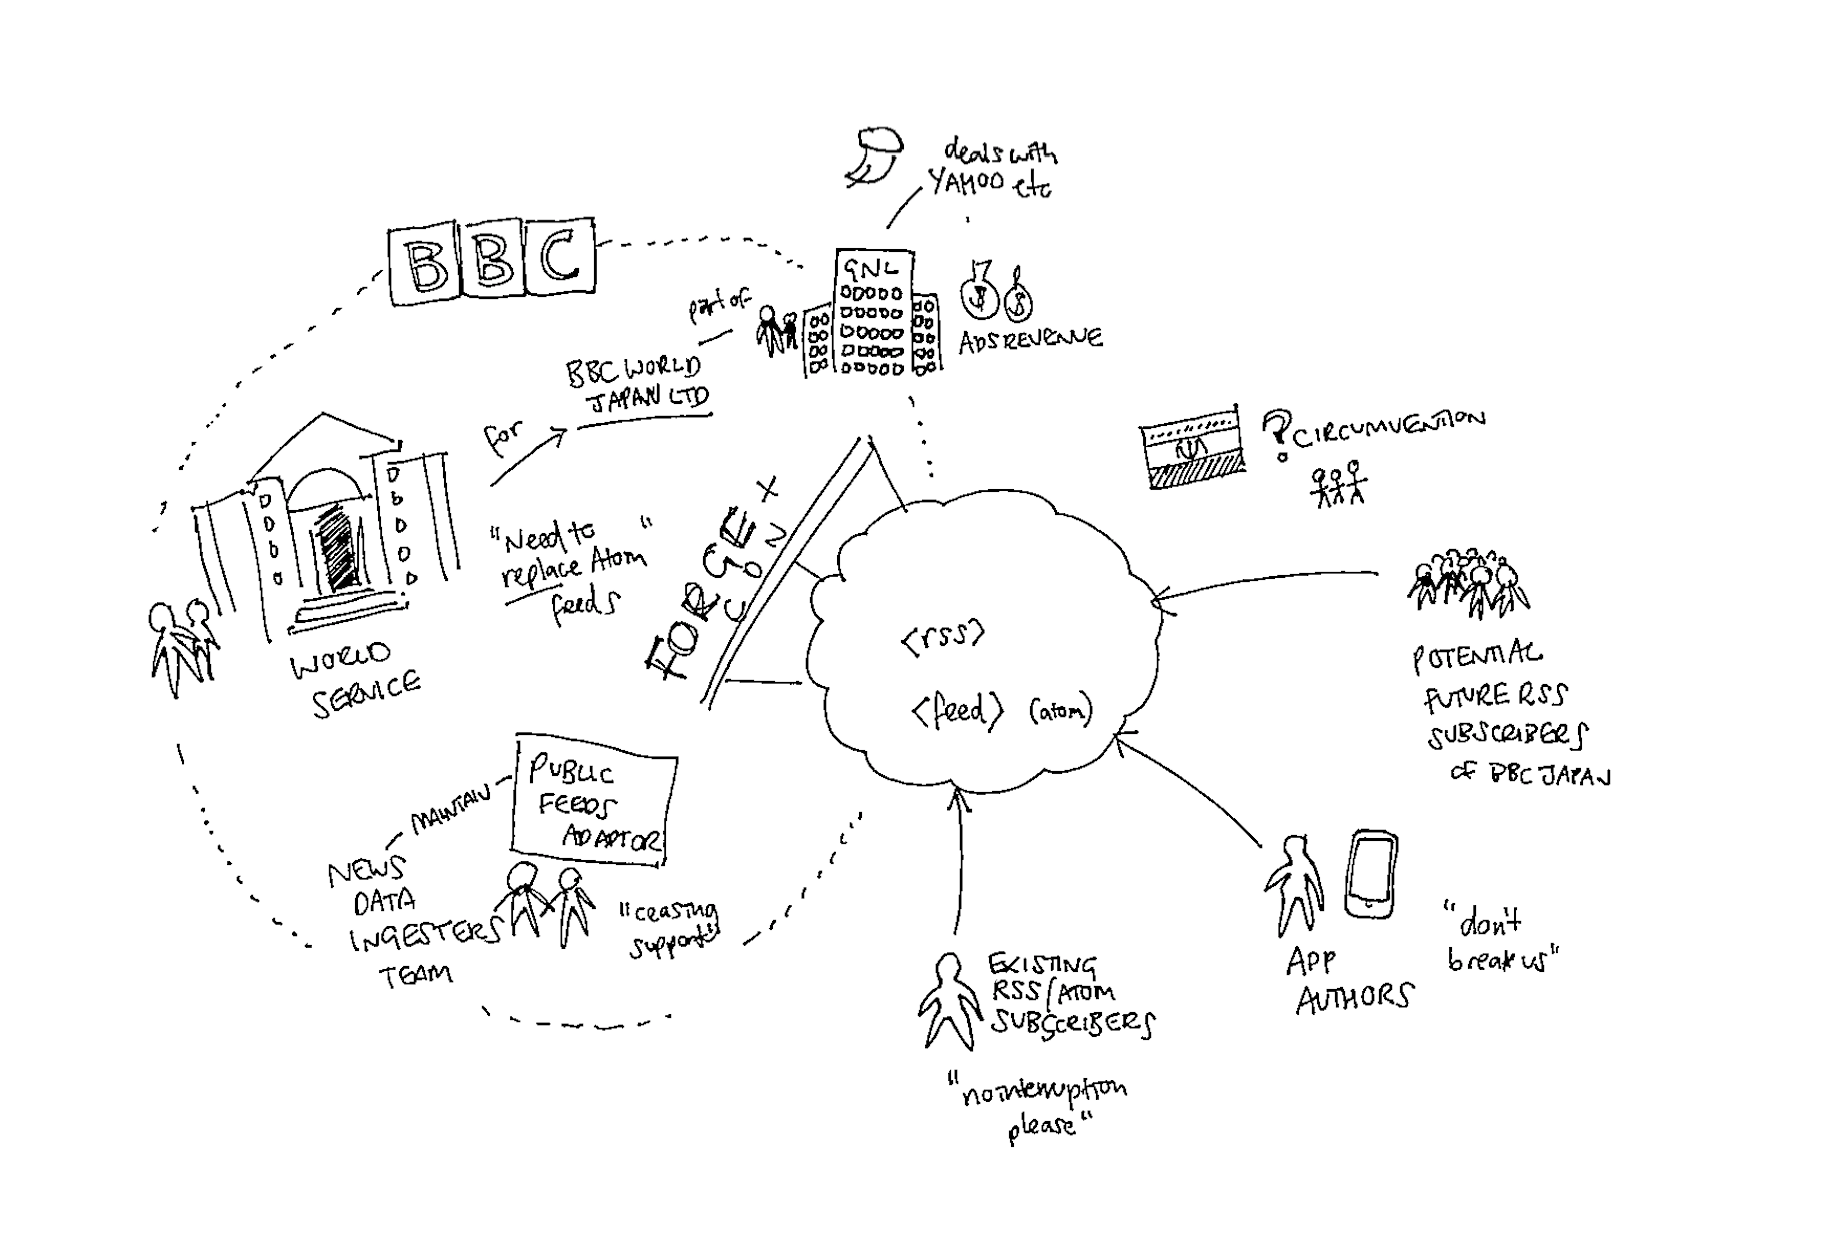
\includegraphics[width=\textwidth]{richpicture.png}
  \caption{Rich Picture of the BBC's problematic situation}
  \label{rich-picture}
\end{figure}

Our rich picture suggests some of the actors whose worldview we should consider. Indeed, SSM's role analysis (known as 'Analysis One') expands the definition of 'issue owner' to be anyone who may be "concerned about or affected by the situation and the outcome" (Checkland and Poulter, p.28). From this perspective, the owners of the issue include the News Product Development Group, the BBC Trust, the Public Feeds Adaptor team and the World Service editorial staff, but members of the public currently subscribed to feeds, builders of third-party apps that consume the feeds, and even potential future users who do not currently use the feeds.

Next, SSM proposes the creation of a number of models showing 'purposeful activity' within a worldview that is made explicit. The starting point for each model is a root definition that describes the system as a statement using the PQR formula (Checkland and Poulter, p.39). Taking one example from the rich picture, we can write the following root definition:

\begin{displayquote}
A system to provide a new web syndication platform for World Service sites by automatically generating and serving up-to-date RSS feeds, in order to allow users to receive updates about new and changed content and therefore contribute to an increase in traffic.
\end{displayquote}

As a further step to enrich our understanding of this system, Soft Systems encourages us to consider the mnemonic CATWOE (Checkland and Poulter, p.42). Through this we might see a transformation (the T) from a deprecated legacy system with no support for the new CMS, to a better-supported and more flexible platform that will meet the BBC's wider needs in years to come. CATWOE offers a distinction between actors (who are involved in the system's activities), owners and customers who are affected by it. This allows us to refine our list of users given earlier.

Finally, we should give consideration to environment (the E of CATWOE). There are several dimensions to this, including the operational environment of the BBC itself, but also the context of the changing landscape of web syndication in the age of Twitter and Facebook. These considerations, and what impact they have on the actors involved, will be reflected in the use case diagrams and other artefacts produced in the next section.

% What about a diagram of an actual SSM purposeful system?
% Add project glossary?

% Stefano did 'Problem space contextualisation' and then 'Design'
% Ross did 'The problem' with 'Design goals' before moving on to Soft Systems

% Hoseyin suggested sections: 'literature review', 'methodology' and 'results'
% See notes from day

\subsection{Project glossary}

\begin{description}

\item [Syndication feed]
A feed of syndication stuff

\item [Subscriber]
blah

\end{description}

\section{Results}

In this section we present a series of UML diagrams that further explore the problematical situation described above. These diagrams are organised according to some of the phases of the software development lifecycle as defined by the Unified Process (UP).

\subsection{Requirements}

From the root definition and list of actors given earlier, we can create the UML use case diagram shown in Figure~\ref{use-cases} which is non-comprehensive depiction of some of the use cases that the system must support. For the purposes of this diagram three actors have been identified, which represent three roles that users of the system may occupy. Further roles could be added in response to later analysis, since as Arlow and Neustadt (p.74) stress, use case modelling is an iterative process. This provisionality applies equally to the system boundary (represented by the black rectangle) that indicates the \textit{subject} of the diagram.

\begin{figure}
  \includegraphics[width=\textwidth]{usecases.png}
  \caption{A use case diagram}
  \label{use-cases}
\end{figure}

In order to describe each use case in more detail, we can use the tabular structure for use case specifications recommended by Arlow and Neustadt, an example of which for one of the use cases shown in Figure~\ref{use-cases} (\texttt{GetFeed}), can be seen in Table~\ref{use-case-detail}. In this use case the primary actor (the one who triggers the use case) is the \texttt{FeedSubscriber}. This use case has one major possible alternative flow, which occurs when the subscriber requests a non-existent feed and is shown in Table~\ref{use-case-alt-detail}. An alternative approach would have been to use the \textit{If} and \textit{Else} keywords within the main flow of Table~\ref{use-case-detail} to describe an alternate flow without creating an entire separate specification.

\begin{table}[]
\begin{center}
\begin{tabular}{ | p{\textwidth} |}
\hline
\multicolumn{1}{|c|}{Use case: GetFeed} \\
\hline
ID: 1 \\
\hline
Brief description: \\
The system return a web syndication feed containing information about content that has recently been created or updated \\
\hline
Primary actors: \\
FeedSubscriber \\
\hline
Secondary actors: \\
None \\
\hline
Preconditions: \\
None \\
\hline
Main flow: \\
1. The use case starts when the FeedSubscriber requests a feed via the network \\
2. The system verifies that the feed exists and has content \\
3. The system generates the feed using the parameters given in the request \\
4. The system serialises the feed is the required format \\
5. The system returns the serialized feed to the FeedSubscriber \\
\hline
Postconditions: \\
None \\
\hline
Alternative flows: \\
GetFeed:MissingFeed \\
\hline
\end{tabular}
\end{center}
\caption{Example of a use case specification}
\label{use-case-detail}
\end{table}

\begin{table}[]
\begin{center}
\begin{tabular}{ | p{\textwidth} |}
\hline
\multicolumn{1}{|c|}{Alternative flow: GetFeed:MissingFeed} \\
\hline
ID: 1.1 \\
\hline
Brief description: \\
The system notifies the user that the requested feed does not exist. \\
\hline
Primary actors: \\
FeedSubscriber \\
\hline
Secondary actors: \\
None \\
\hline
Preconditions: \\
None \\
\hline
Alternative flow: \\
1. The alternative flow begings after step 2 of the main flow. \\
2. The system displays an HTML error page to the FeedSubcriber \\
\hline
Postconditions: \\
None \\
\hline
\end{tabular}
\end{center}
\caption{Example of a use case alternative flow specification}
\label{use-case-alt-detail}
\end{table}

\clearpage
\subsection{Design}

\begin{figure}
  \begin{center}
    \includegraphics[width=\textwidth]{sequence.png}
  \end{center}
  \label{sequence}
  \caption{A sequence diagram}
\end{figure}

\section{Evaluation}
Evaluation and analysis.

% Rich pictures are never finished, they should evolve as enquiry progresses (LFA p25)

\section{Conclusion}
Nothing besides remains.

\begin{thebibliography}{9}

\bibitem{bbc2013} 
British Broadcasting Corporation, 2013.
\textit{BBC announces ambition to double global audience to 500 million} [online].
Available from: http://www.bbc.co.uk/mediacentre/latestnews/2013/dg-global-audience [Accessed 24 June 2016].

\bibitem{w3c1997} 
World Wide Web Consortium, 1997.
\textit{Channel Definition Format (CDF)} [online].
Available from: https://www.w3.org/TR/NOTE-CDFsubmit.html
[Accessed 24 July 2016].

\bibitem{checkland1990}
Checkland, P. and Scholes, J. 1990.
\textit{Soft Systems Methodology in Action}.
Chichester: John Wiley

\bibitem{checkland2006} 
Checkland, P. and Poulter, J., 2006.
\textit{Learning for Action: A Short Definitive Account of Soft Systems Methodology and its use for Practitioners, Teachers and Students}.
Chichester: John Wiley

\bibitem{arlow} 
Arlow, J. and Neustadt, I., 2005.
\textit{UML 2 and the Unified Process}. Second Edition. Upper Saddle River, NJ: Addison-Wesley

\end{thebibliography}

\end{document}
